\documentclass[11pt,a4paper]{article}
\usepackage[margin=2.5cm]{geometry}
\usepackage{graphicx}
\usepackage{tikz}
\usetikzlibrary{shapes.geometric,arrows.meta,positioning}
\usepackage{listings}
\usepackage{xcolor}
\usepackage{booktabs}
\usepackage{caption}
\usepackage[hidelinks]{hyperref}

\lstset{basicstyle=\ttfamily\small, frame=tb, columns=fullflexible, keepspaces=true}

\title{Operating Systems Lab 3: A User-Level Thread Scheduler}
\author{Mei Tanaka (s2290413)}
\date{Submitted 6 November 2026}

\begin{document}
\maketitle
\tableofcontents
\listoffigures
\listoftables

\section{Introduction}
This report describes a round-robin scheduler for user-level threads implemented with
\texttt{ucontext}.\footnote{See \texttt{man 3 makecontext}.} Threads yield voluntarily or
are preempted by a \texttt{SIGALRM} timer every 10\,ms.

\section{Design}
Figure~\ref{fig:states} shows the thread state machine.

\begin{figure}[h]
\centering
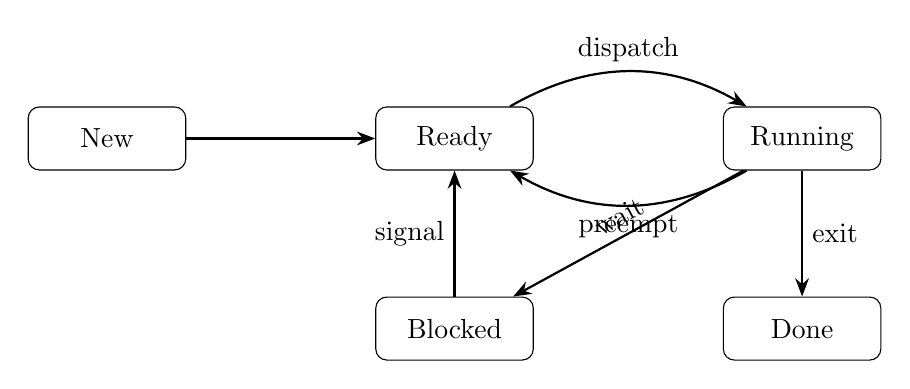
\begin{tikzpicture}[node distance=1.6cm and 2.4cm,
  st/.style={rectangle, rounded corners, draw, minimum width=2cm, minimum height=0.8cm},
  arr/.style={-{Stealth}, thick}]
  \node[st] (new) {New};
  \node[st, right=of new] (ready) {Ready};
  \node[st, right=of ready] (run) {Running};
  \node[st, below=of ready] (blk) {Blocked};
  \node[st, below=of run] (done) {Done};
  \draw[arr] (new) -- (ready);
  \draw[arr] (ready) to[bend left] node[above] {dispatch} (run);
  \draw[arr] (run) to[bend left] node[below] {preempt} (ready);
  \draw[arr] (run) -- node[right] {exit} (done);
  \draw[arr] (run) -- node[sloped, above] {wait} (blk);
  \draw[arr] (blk) -- node[left] {signal} (ready);
\end{tikzpicture}
\caption{Thread states and transitions.}
\label{fig:states}
\end{figure}

The core of the scheduler is the context switch:

\begin{lstlisting}[language=C]
void schedule(void) {
    thread_t *prev = current;
    current = queue_pop(&ready_queue);
    if (prev->state == RUNNING) {
        prev->state = READY;
        queue_push(&ready_queue, prev);
    }
    current->state = RUNNING;
    swapcontext(&prev->ctx, &current->ctx);
}
\end{lstlisting}

\section{Evaluation}
\begin{table}[h]
\centering
\caption{Context-switch latency (median of 10\,000 switches).}
\label{tab:latency}
\begin{tabular}{lr}
\toprule
Mechanism & Latency (ns) \\
\midrule
\texttt{swapcontext} & 412 \\
Hand-written assembly & 38 \\
\texttt{pthread} yield & 1\,950 \\
\bottomrule
\end{tabular}
\end{table}

As Table~\ref{tab:latency} shows, \texttt{swapcontext} is slow because it saves and
restores the signal mask with a system call.

\appendix
\section{Build instructions}
Run \texttt{make} in the project root, then \texttt{./bench 10000}.

\section{Test output}
\begin{lstlisting}
$ ./test_sched
[ok] create/join 100 threads
[ok] preemption fairness (max skew 3%)
[ok] mutex under contention
\end{lstlisting}

\end{document}
